\documentclass[twocolumn]{article}

% Margins
\topmargin=-0.45in
\evensidemargin=0in
\oddsidemargin=0in
\textwidth=6.5in
\textheight=9.0in
\headsep=0.25in

\linespread{1.5}

\usepackage{ctex}
\usepackage{fontspec}
\usepackage{inputenc}
\usepackage{float}
\usepackage{multirow}
\usepackage{graphicx}
\usepackage{geometry}
\usepackage{subfigure}
\usepackage{amsmath,amsfonts,amsthm,amssymb}
\usepackage{listings}
\usepackage[bottom]{footmisc}
%\usepackage{abstract}
%\usepackage[hyperref=true,sorting=none]{biblatex}
\usepackage[english]{babel}
\usepackage{hyperref} %[hidelinks]
\usepackage{algorithm}
%\usepackage{algorithmicx}
%\usepackage{algpseudocode}

\geometry{left=1.4cm,right=1.4cm,top=2.5cm,bottom=2.5cm}

\title{\textbf{Automatic Model Selection Techniques for RBF Network}}
\author{高枫\ 2015011208 \\
gaof15@mails.tsinghua.edu.cn}
\date{}

\begin{document}

\maketitle

\section*{\centering Abstract}

本文基于Reversible Jump MCMC模型选择技术,横向研究了Simulated  Annealing和AIC等方法在Radial Basis Function(RBF)网络选择问题上的应用性能,此外,还将RJ-MCMC方法与针对RBF网络模型进行优化后的Orthogonal Least Squares Learning(OLS)方法进行了比较,从而给出了RBF网络模型自动选择技术的综合性说明。

% \noindent 
\textit{\textbf{Keyword}:\ RBF Network, Metropolis-Hastings, RJMCMC, Simulated Annealing, AIC, OLS}

\section*{\centering I. Introduction}

Radial\ Basis\ Function(RBF)网络是一种经典的神经网络结构,由于RBF网络能够逼近任意的非线性函数,RBF网络通常被应用于处理系统内难以解析的规律性,具有良好的泛化能力,并有很快的学习收敛速度,现已成功应用于多种场景。而如何选择RBF网络模型的参数便成为了实际应用RBF模型的首要困难。

经典的RBF模型选择标准有很多种,如Akaike的AIC准则\cite{1100705}、Schwarz的MDL准则\cite{MDL},Andrieu的Reversible\ Jump\ MCMC\ Simulated\ Annealing(RJMCMCSA)方法\cite{DBLP}等,其中AIC等准则可以用来评判不同模型间的优劣,而RJMCMCSA方法中使用RJMCMC过程进行模型更新,然后用模拟退火算法进行模型选择。使用RJMCMC方法的好处在于我们可以使用任意维度的初始模型开始训练,算法会自动在不同模型间跳转,直到找到“最优”模型。鉴于这种方法的优越性,本文中将AIC准则与RJMCMC方法相结合,比较了其与RJMCMCSA方法在RBF模型选择问题上的性能。此外,为了更全面地研究RBF模型选择方法,本文中还将展示RJMCMC方法替换成了Orthogonal\ Least\ Squares(OLS)方法\cite{80341}之后的选择性能。总而言之,本文的目标在于全面细致地展示当下几种RBF模型选择方法,并将不同方法间的性能优劣进行比较。

本文的结构安排如下,$II$中将介绍一种传统的MCMC方法,Metropolis-Hastings算法,以及改进之后的RJMCMC方法,在$III$中对RBF网络模型进行简单的介绍,然后在$IV$中分别介绍SA、AIC方法以及OLS方法,并阐述其实现过程,$V$中会介绍将上述几种方法实际测试之后的结果,分析比较不同方法间的性能差异,最后在$VI$将对上述全部RBF模型选择方法进行总结。

\section*{\centering II. Markov Chain Monte Carlo}

\subsection*{A. Standard MCMC}
马尔科夫蒙特卡洛(Markov Chain Monte Carlo, MCMC) 方法,是用一组Markov\ Chain从随机分布中取样的算法,得到的序列可用于估计该概率分布或计算积分等。但不同于以往的蒙特卡洛integration是统计独立的,MCMC中的是统计相关的。

在采用MCMC方法时马尔科夫链转移核的构造至关重要,不同的转移核构造方法将产生不同的MCMC方法,目前常用的MCMC方法主要有两种Gibbs抽样和Metropo-Lis-Hastings算法(Algorithm 1)\cite{Metropolis1953}\cite{wiki:Metropolis–Hastings_algorithm}。

本文将以Metropolis-Hastings算法为主进行介绍,后面提到的RJMCMC方法就是MH方法的一种扩展算法,其他很多的MCMC方法也都基于这种基本算法。Metropolis-Hastings算法一般用于从多变量分布中采样,对于单变量分布而言,常会使用自适应判别采样(adaptive\ rejection\ sampling)等其他能抽取独立样本的方法,而不会出现MCMC中样本自相关的问题。

\begin{algorithm}[H]
\caption{Metropolis-Hastings algorithms}
\textbf{Initialization}:

    \textbf{a.} Pick an initial state $x_0$
    
    \textbf{b.} Set $t = 0$
        
\textbf{Iteration t}:
    
    \textbf{a. Generate}: randomly generate a candidate state $x'$ according to $g(x'|x_t)$
    
    \textbf{b. Calculate}: calculate the acceptance probability $A(x'|x_t)=\min (1, \frac{P(x')g(x_t|x')}{P(x)g(x'|x_t)})$
    
    \textbf{c. Accept or Reject}:
    
    \ \ \ \ a. generate a uniform random number $u\in [0,1]$
    
    \ \ \ \ b. if $u\leq A(x'|x_t)$, accept the new state and set $x_{t+1}=x'$
    
    \ \ \ \ c. if $u>A(x'|x_t)$, reject the new state and set $x_{t+1}=x_t$
    
    \textbf{d.\ Increment}: set $t=t+1$
    
\end{algorithm}

\subsection*{B. Reversible Jump MCMC}

可逆跳跃马尔科夫蒙特卡洛(Reversible Jump Markov Chain Monto Carlo,RJMCMC)方法(Algorithm 2)\cite{doi:10.1093/biomet/82.4.711}\cite{Andrieu99robustfull}是上一小节中介绍的标准MCMC方法的扩展,其好处在于可以模拟变维空间中的后验分布,即使模型参数是未知的,我们仍然可以进行模拟采样的过程。因此这种方法可以应用于各种复杂的模型选择问题,RBF网络模型的选择就是其重要的应用场景之一。

在RJMCMC过程中,每次先在同一维度的模型中更新模型参数,然后再在不同维度的模型间跳转,然后用接受概率决定是否更新模型。这种方法与传统MCMC方法的区别就在于它会在不同模型间跳转,这就使得变维空间中的抽样变得可实现,从而简化了模型选择算法。

\section*{\centering III. RBF Network}

径向基函数网络(Radial basis function network,RBF network)是一种使用径向基函数作为激活函数的人工神经网络。径向基函数网络的输出是输入的径向基函数和神经元参数的线性组合。

径向基函数网络通常有三层:输入层、隐藏层和一个非线性激活函数和线性径向基神经网络输出层。输入可以被建模为实数向量。输出是输入向量的一个标量函数。

\begin{figure}[H]
  \centering
  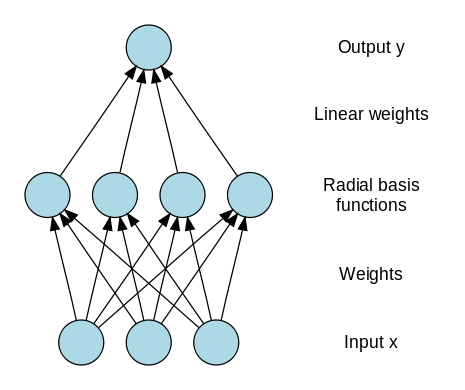
\includegraphics[width=2.5in]{465px-Radial_funktion_network.png}
  \caption{Architecture of a radial basis function network.An input vector $x$ is used as input to all radial basis functions, each with different parameters. The output of the network is a linear combination of the outputs from radial basis functions.}
\end{figure}

RBF模型可以简单表示为以下形式\cite{DBLP}:$$y_{N\times c} = D(\mu_{k\times d}, x_{N\times d})\alpha_{(1+d+k)\times c} + n_{N\times c}$$

y为观测样本,N为样本点数,c为每个样本点的维度,x为N个观测样本点对应的变量,d为每个变量的维度,矩阵D有如下形式
$$D=\begin{bmatrix}

    1 & x_{1,1} & \dots & x_{1,d} & \phi(x_1, \mu_1) & \dots & \phi(x_1, \mu_k) \\
    1 & x_{2,1} & \dots & x_{2,d} & \phi(x_2, \mu_1) & \dots & \phi(x_2, \mu_k) \\
    \vdots & \vdots & \ddots & \vdots & \vdots & \ddots & \vdots \\
    1 & x_{N,1} & \dots & x_{N,d} & \phi(x_N, \mu_1) & \dots & \phi(x_N, \mu_k) \\

\end{bmatrix}$$

%$$\sigma_i^2=\frac{1}{N}y_{1:N, i}^T P y_{1:N, i} = \frac{1}{N}y_{1:N, i}^T(I_N-D[D^TD]^{-1}D^T)y_{1:N, i}$$

%$$\alpha_{1:m, i} = [D^TD]^{-1}D^Ty_{1:N, i}$$

$\phi(x,\mu)$表示RBF函数,k为RBF函数的个数,$\mu$为函数的中心,$\alpha$为加权系数,n是服从高斯分布的白噪声,$n_i\sim\mathcal{N}(0,\sigma_i^2),i=1,2,...,c$。RBF模型的参数集合可用$\mathcal{M}_s=(\mu, \alpha, \sigma^2, k)=(\theta, k)$表示。

\section*{\centering IV. Model Selection for RBFN}

\subsection*{A. Reversible Jump Simulated Annealing}

Reversible Jump MCMC Simulated Annealing算法\cite{DBLP}是Andrieu提出的一种结合了RJMCMC和模拟退火算法的模型选择算法。其过程见Algorithm 2。模拟退火(Simulated Annealing)\cite{1983Sci...220..671K}是一种通用概率算法,用来在固定时间内寻求在一个大的搜寻空间内找到的最优解。

使用了模拟退火算法的MH步骤中的接受概率变为

$$A_{SA} = \min \{1, \frac{\pi^{(1/T_i-1)}(z^*)}{\pi^{(1/T_i-1)}(z)}\}$$

其中$T_i$是递减的cooling schedule,满足$lim_{i\rightarrow \infty}T_i = 0$,$\pi(z)$是样本的随机分布。

在RBF模型选择问题中,共有五种Move方式,分别是Birth Move, Death Move, Split Move, Merge Move和Update,每次迭代中发生这几种move的概率分别为$b_k$, $d_k$, $s_k$, $m_k$和$u_k$,满足$b_k+d_k+s_k+m_k+u_k = 1$。其中Birth Move和Split Move允许RBF网络的隐层维度从k增长到k+1,Death Move和Merge Move允许维度从k减少到k-1。

\begin{algorithm}[H]
\caption{Reversible Jump Simulated Annealing}
\textbf{Initialization}:

Set $(k^{(0)}, \theta^{(0)}) \in \Theta$

\textbf{Iteration i}:

a. Sampling u~U[0,1] and set the temperature with a cooling schedule

b. if $u \leq b_{k^{(i)}}$

\ \ \ \ \ \ \ \ do "birth" move

\ \ \ \ else if $u \leq b_{k^{(i)}} + d_{k^{(i)}}$

\ \ \ \ \ \ \ \ do "death" move

\ \ \ \ else if $u \leq b_{k^{(i)}} + d_{k^{(i)}} + s_{k^{(i)}}$

\ \ \ \ \ \ \ \ do "split" move

\ \ \ \ else if $u \leq b_{k^{(i)}} + d_{k^{(i)}} + s_{k^{(i)}} + m_{k^{(i)}}$

\ \ \ \ \ \ \ \ do "merge" move

\ \ \ \ else

\ \ \ \ \ \ \ \ update the RBF centres

c. Perform an MH step with the annealed acceptance ratio.

d. i = i + 1

\end{algorithm}

\subsection*{B. Akaike Information Criterion}

赤池信息量准则(Akaike information criterion, AIC)\cite{1100705}是评估统计模型的复杂度和衡量统计模型“拟合”资料之优良性的一种标准。AIC准则建立在信息熵的概念基础上,目标在于选择可以最好地解释数据但包含最少自由参数的模型。

在一般情况下,AIC可以表示为

$$AIC = 2k - 2\ln(L)$$

其中,k是参数的数量,L是似然函数。

可以看出,增加自有参数的数量可以提高拟合的优良性,而AIC鼓励拟合的优良性但尽量避免出现过拟合的情况。所以优先考虑的模型应该是AIC值小的那个。

\subsection*{C. Orthogonal Least Squares Learning}

正交最小二乘(Orthogonal Least Squares, OLS)算法\cite{soton251147}最早在20世纪80年代后期提出,主要用于非线性系统建模。后来Chen又在\cite{80341}中提出将OLS方法应用于RBF网络模型的选择问题。为了最小化均方误差,OLS算法逐项寻求回归模型,力求每一项都能够最小化回归残差。因为每一个回归项都会影响以后回归项的选择,所以每一项都会影响整个模型的性能。而OLS方法是一种贪心算法,只寻求当前步骤最优解,而忽略它对下一步的影响,即每步并非全局最优。

下面我将对一维输出的OLS算法进行描述,对于多维输出可以将下述算法进行平凡地推广。对于给定输入x时,网络的输出为

$$y = P\Theta + E$$

其中,

$y = [y(1), y(2), ..., y(N)]$

$P = [p_1, p_2, ..., p_M], p_1 = [p_i(1), ..., p_i(N)]^T, \\p_i(t) = p_i(x(t)), 1\leq i \leq M$

$\Theta = [\theta_1, ..., \theta_M]^T$

$E = [\epsilon(1), ..., \epsilon(N)]^T$

M是RBF网络中隐层的维度,即RBF核函数的个数,N是输入的样本数。

上述的回归矩阵$P$可被分解为

$$P=WA$$

其中$A$为$M\times M$的上三角阵,且对角元都为1

$$A = \begin{bmatrix}
    1 & \alpha_{12} & \alpha_{13} & \dots  & \alpha_{1M} \\
    0 & 1 & \alpha_{23} & \dots  & \alpha_{2M} \\
    0 & 0 & 1 & \dots  & \alpha_{3M} \\
    \vdots & \vdots & \vdots & \ddots & \vdots \\
    0 & \dots & 0 & 0  & 1
\end{bmatrix}$$

W为$N\times M$的矩阵,且其列向量是彼此正交的。

则进行矩阵分解后,$y$的表达式变为

$$y = Wg + E$$

定义误差减小率为

$$[err]_i = g_i^2w_i^Tw_i/(y^Ty)$$

则训练过程如Algorithm 3所示。

\begin{algorithm}[htb]
\caption{Orthogonal Least Squares}
\textbf{At the first step, for $1 \leq i \leq M$}

\ \ \ \ \ \ \ \ $w_1^(i)=p_i$

\ \ \ \ \ \ \ \ $g_1^(i)=(w_1^{(i)})^Ty/((w_1^{(i)})^Tw_1^{(i)})$

\ \ \ \ \ \ \ \ $[err]_1^{(i)}=(g_1^{(i)})^2(w_1^{(i)})^Tw_1^{(i)}/(y^Ty)$

Find

\ \ \ \ \ \ \ \ $[err]_1^{(i_1)}=\max\{[err]_1^{(i)}, 1\leq i \leq M\}$

and select

\ \ \ \ \ \ \ \ $w_1 = w_1^{(i_1)}=p_{i_1}$

\textbf{At the kth step where $k\geq 2$, for $1\leq i\leq M, i\neq i_1, ..., i\neq i_{k-1}$, }

\ \ \ \ \ \ \ \ $\alpha_{jk}^{(i)}=w_j^Tp_i/(w_j^Tw_j), 1\leq j<k$

\ \ \ \ \ \ \ \ $w_k^{(i)}=p_i-\sum_{j=1}^{k-1}\alpha_{jk}^{(i)}w_j$

\ \ \ \ \ \ \ \ $g_k^(i)=(w_k^{(i)})^Ty/((w_k^{(i)})^Tw_k^{(i)})$

\ \ \ \ \ \ \ \ $[err]_k^{(i)}=(g_k^{(i)})^2(w_k^{(i)})^Tw_k^{(i)}/(y^Ty)$

Find

\ \ \ \ \ \ \ \ $[err]_k^{(i_k)}=\max\{[err]_k^{(i)}, 1\leq i \leq M, i\neq i_1, ..., i\neq i_{k-1}\}$

and select

\ \ \ \ \ \ \ \ $w_k = w_k^{(i_k)}=p_{i_k}-\sum_{j=1}^{k-1}\alpha_{jk}^{(i)}w_j$

\textbf{The procedure is terminated at the $M_sth$ step}

\ \ \ \ \ \ \ \ $1-\sum_{j=1}^{M_s}[err]_j<\rho$

\end{algorithm}

\section*{\centering V. Experiment}

\subsection*{A. Metropolis-Hastings Simulation}

使用MH算法对下述二维高斯分布进行随机采样,并利用采样结果估计二维高斯分布的相关系数$\rho$

$$\mathcal{N}\left\{
\begin{pmatrix}
x_1 \\
x_2
\end{pmatrix}|
\begin{pmatrix}
5 \\
10
\end{pmatrix},
\begin{pmatrix}
1 & -1 \\
-1 & 4
\end{pmatrix}
\right\} $$

由于算法开始运行时采样并不准确,因此舍弃前面的200个采样点,使用后面的采样点进行估计。设置最大迭代次数为50000次。对不同的建议分布选取绘制其相对误差和相关系数的变化曲线。

1. 取建议分布的协方差矩阵与已知的二维高斯分布相同,均值为满足二维高斯分布的随机向量,得到loss和$\rho$的变化曲线如Figure 2所示。

\begin{figure}[H]
  \centering
  \subfigure[$loss$]{
    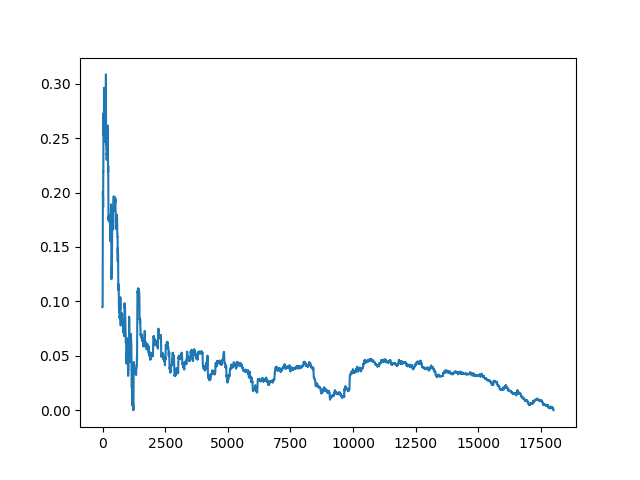
\includegraphics[width=1.7in]{loss_mh.png}}
  \hspace{0in}
  \subfigure[$\rho$]{
    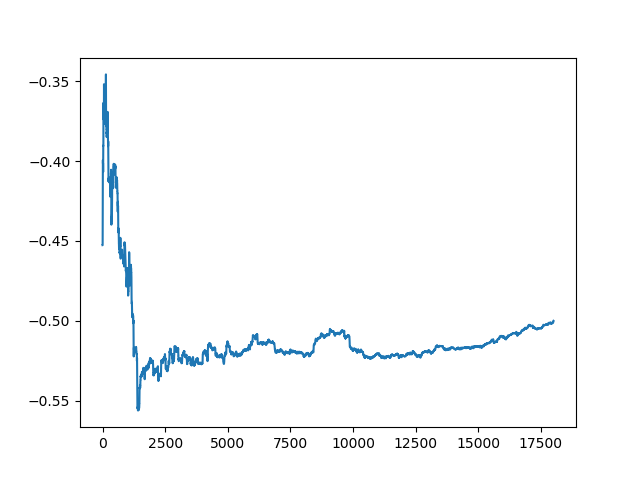
\includegraphics[width=1.7in]{Rho.png}}
  \caption{Metropolis-Hastings Simulation($\Sigma$)}
\end{figure}

2. 取建议分布的均值与1中选取方式相同,协方差矩阵为原矩阵的2倍,得到loss和$\rho$的变化曲线如Figure 3所示。

\begin{figure}[H]
  \centering
  \subfigure[$loss$]{
    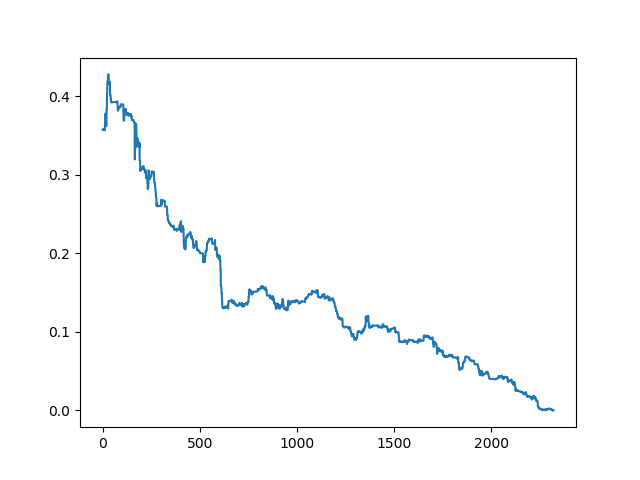
\includegraphics[width=1.7in]{loss_mh_2.png}}
  \hspace{0in}
  \subfigure[$\rho$]{
    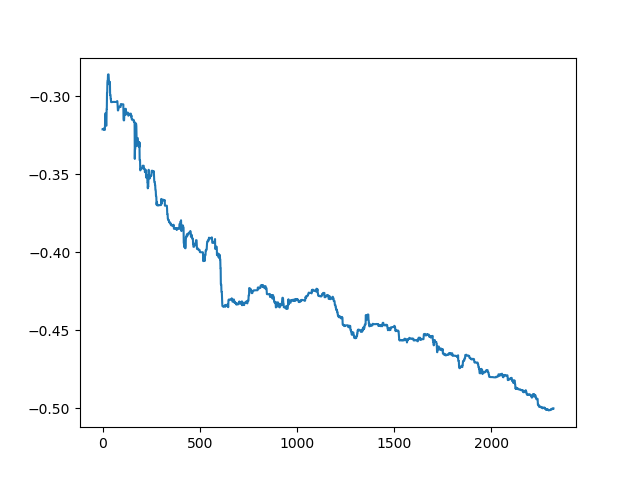
\includegraphics[width=1.7in]{Rho_2.png}}
  \caption{Metropolis-Hastings Simulation($2\Sigma$)}
\end{figure}

3. 取建议分布的均值与1中选取方式相同,协方差矩阵为原矩阵的4倍,得到loss和$\rho$的变化曲线如Figure 4所示。

\begin{figure}[H]
  \centering
  \subfigure[$loss$]{
    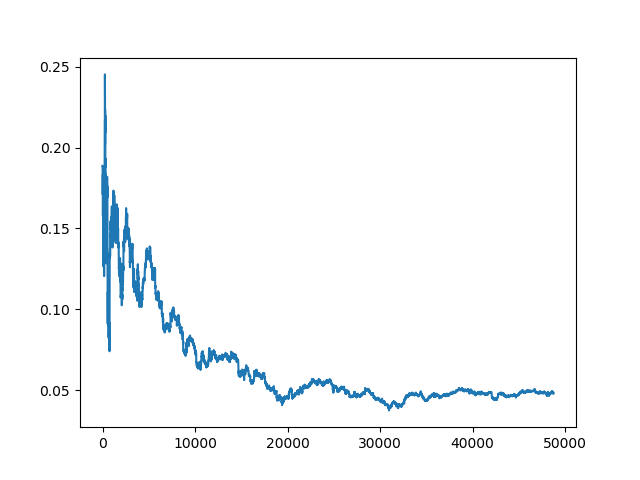
\includegraphics[width=1.7in]{loss_mh_1.png}}
  \hspace{0in}
  \subfigure[$\rho$]{
    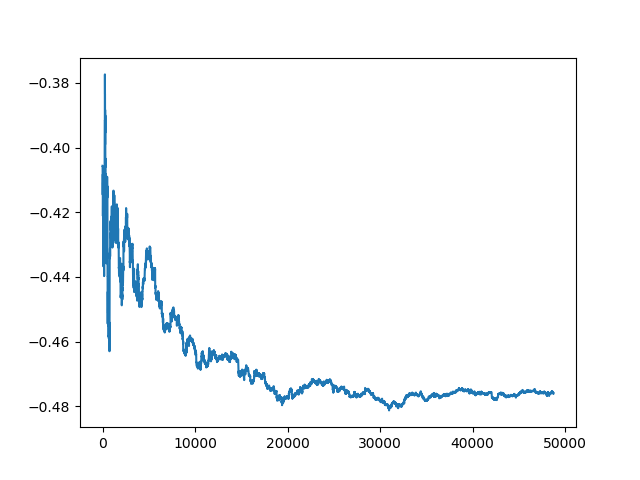
\includegraphics[width=1.7in]{Rho_1.png}}
  \caption{Metropolis-Hastings Simulation($4\Sigma$)}
\end{figure}

将上述三个实验的数据整理成Tabel 1,可以看出,当建议分布比较接近目标分布时,收敛速度较快,且最后拟合的效果比较好,而如果建议分布与目标分布区别较大时,则不能以很快的速度收敛。

\begin{table}[H]
\centering
\begin{tabular}{c|ccc}
\hline
$\Sigma_Q$ & \#iter & $\rho$ & loss \\
\hline
$\Sigma$ & 18846 & -0.5000 & 0.0001 \\
$2\Sigma$ & 3336 & -0.5000 & 0.0000 \\
$4\Sigma$ & 50000 & -0.4759 & 0.0482 \\
\hline
\end{tabular}
\caption{Metropolis-Hastings Simulation}
\end{table}

\subsubsection*{B. Reversible Jump MCMC Simulation}

\cite{doi:10.1093/biomet/82.4.711}中在介绍RJMCMC过程时,选择了以British Coal Mine Disaster数据进行训练,期望拟合出一个分段常值函数,为验证其可靠性,本次选择使用相同的数据集进行训练。Figure 5中为数据集的可视化图形。

\begin{figure}[H]
  \centering
  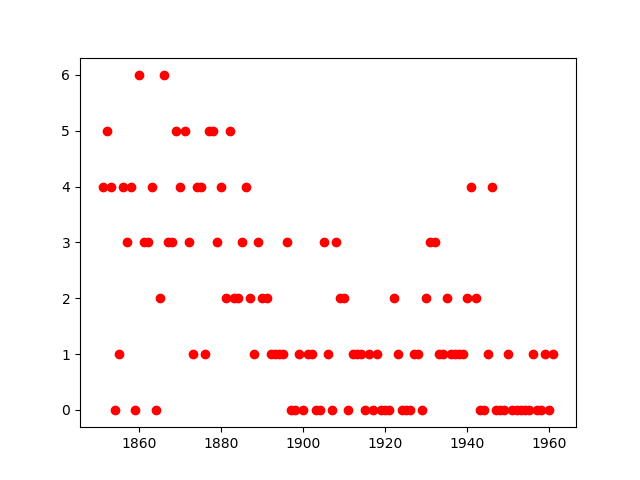
\includegraphics[width=2.5in]{coal_data.png}
  \caption{British Coal Mine Disaster Data}
\end{figure}

我们期望的分布为一个分段常值的函数,在给定区间中,k为函数的step数,对于每个给定的k,各个step的起止位置和高度都是未知的,从而可以转化为变维空间中的模型选择问题,选择使用RJMCMC方法进行训练。

本实验中选择使用均方误差(Mean Square Error, MSE),得到的loss变化曲线如Figure 6所示。可以看出,使用RJMCMC可以快速地将loss降低,最后能够得到一个稳定,且与期待分布十分接近的模型。

\begin{figure}[H]
  \centering
  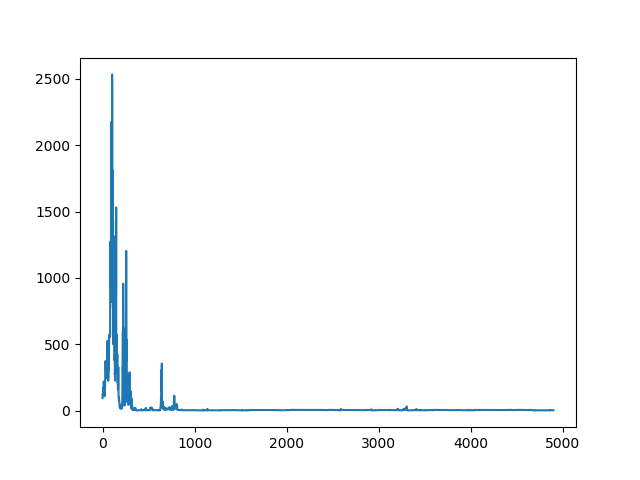
\includegraphics[width=2.5in]{loss_rjmcmc.png}
  \caption{Loss Curve in RJMCMC Simulation}
\end{figure}

\subsection*{C. Model Selection Techniques for RBFN}

本小节中将分别给出使用RJMCMC+SA, RJMCMC+AIC, OLS方法,在给定的两组数据集上的训练结果。为检验训练出的模型在未知数据上的拟合效果,每次训练中随机选取200个数据点组成验证集(Validation Set),并分别输出模型在训练集和验证集中的loss值(此处以及后文所述实验均选择均方误差作为loss)。此外,为了减少数据中的奇异点对训练造成的影响,删除其中y值最大和最小的各两点,即原数据集中共1000个样本,参与训练和验证的样本有996个,其中训练样本796个,验证样本200个。

\subsubsection*{1. RJMCMC+SA}

在RJMCMCSA的训练过程中,选择Gauss Kernel作为RBF函数,则根据IV.A中所述,我们只需选择出使模型最优的RBF函数中心矩阵$\Phi$即可。

使用RJMCMCSA方法在data1和data2两个数据集中分别进行训练,设置最大迭代次数为2000次。得到loss曲线如Figure 6中所示。其中(b)为data2训练过程中的全部loss曲线,(c)为data2去掉前20个点之后的loss曲线。将RJMCMCSA方法分别在两个数据集上的时间开销及训练结果整理成Table 2,其中loss为最终模型在全部996个样本上的均方误差。

\begin{figure}[H]
  \centering
  \subfigure[loss for data 1]{
    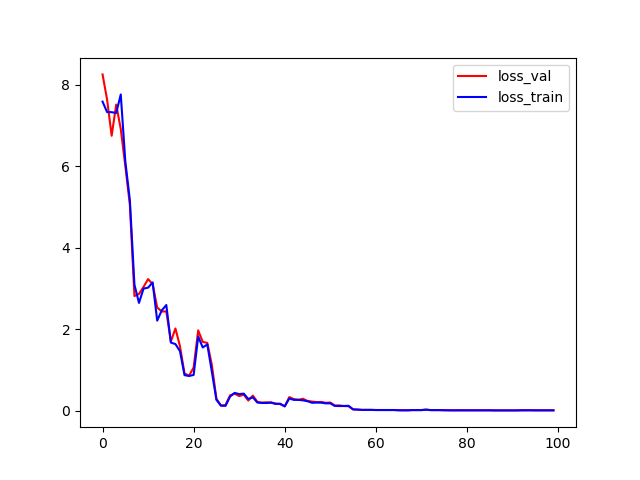
\includegraphics[width=2.5in]{loss1_sa.png}}
  \hspace{0in}
  \subfigure[loss for data 2]{
    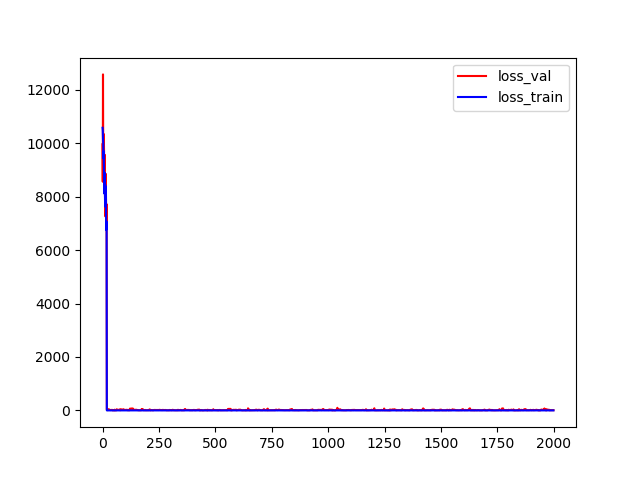
\includegraphics[width=2.5in]{loss2_sa.png}}
  \hspace{0in}
  \subfigure[loss for data 2(without the first 20\ points)]{
    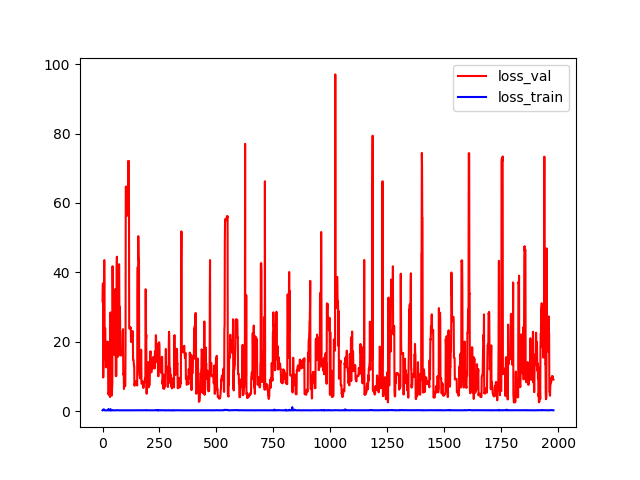
\includegraphics[width=2.5in]{newloss2_sa.png}}
  \caption{Loss Curve for RJMCMC-SA method}
\end{figure}

从loss曲线中可以看出,使用RJMCMCSA方法能够使loss迅速地下降到较低的值。不过也可以看出,RJMCMCSA方法虽然能够得到一个比较优秀的模型选择结果,但是对于较为复杂的数据模型,RJMCMCSA方法的结果波动性较大。在此次实验中,data1的训练结果要远好于data2的训练结果。

\begin{table}[htb]
\centering
\begin{tabular}{c|cccc}
\hline
DataSet & k & \#iter & time & totalLoss \\
\hline
data1 & 31 & 100 & 39.3025s & 0.00469 \\
data2 & 261 & 2000 & 4.1444h & 0.26107 \\
\hline
\end{tabular}
\caption{RJMCMC-SA Experiments}
\end{table}

\begin{table}[htb]
\centering
\begin{tabular}{c|cccc}
\hline
DataSet & k & \#iter & time & totalLoss \\
\hline
data1 & 38 & 146 & 141.1047s & 0.00366 \\
data2 & 280 & 2000 & 4.6632h & 0.23303 \\
\hline
\end{tabular}
\caption{RJMCMC-AIC Experiments}
\end{table}

\begin{table}[H]
\centering
\begin{tabular}{c|cccc}
\hline
DataSet & k & \#iter & time & totalLoss \\
\hline
data1 & 42 & 43 & 13.6006s & 0.00249 \\
data2 & 159 & 160 & 83.9666s & 21.26043 \\
\hline
\end{tabular}
\caption{OLS Experiments}
\end{table}

\begin{table}[H]
\centering
\begin{tabular}{c|cccc}
\hline
Method & k & totalLoss & trainLoss & valLoss \\
\hline
SA & 31 & 0.00469 & 0.00476 & 0.00471 \\
AIC & 38 & 0.00366 & 0.00368 & 0.00376 \\
OLS & 42 & 0.00249 & 0.00244 & 0.00173 \\
\hline
\end{tabular}
\caption{Data1 Experiments for All Methods}
\end{table}

\begin{table}[H]
\centering
\begin{tabular}{c|cccc}
\hline
Method & k & totalLoss & trainLoss & valLoss \\
\hline
SA & 261 & 0.26107 & 0.23415 & 177.34351 \\
AIC & 280 & 0.23303 & 0.22801 & 9.07621 \\
OLS & 159 & 21.26043 & 0.27269 & 0.21333 \\
\hline
\end{tabular}
\caption{Data2 Experiments for All Methods}
\end{table}

\subsubsection*{2. RJMCMC+AIC}

RJMCMC+AIC的实验过程与RJMCMCSA的实验过程基本相同,只不过将其中模拟退火的过程换成了使用AIC准则进行模型更新的选择判定。

使用RJMCMCAIC方法在data1和data2两个数据集中分别进行训练,设置最大迭代次数为2000次。得到loss曲线如Figure 7中所示。其中(b)为data2训练过程中的全部loss曲线,(c)为data2去掉前10个点之后的loss曲线。将RJMCMCSA方法分别在两个数据集上的时间开销及训练结果整理成Table 3,其中loss为最终模型在全部996个样本上的均方误差。

\begin{figure}[H]
  \centering
  \subfigure[loss for data 1]{
    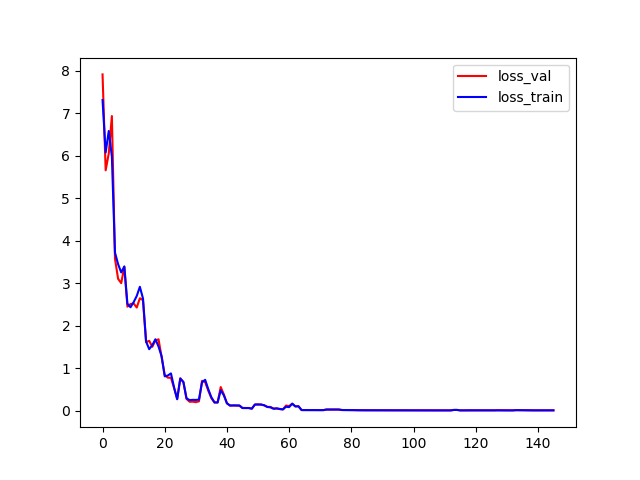
\includegraphics[width=2.5in]{loss1_aic.png}}
  \hspace{0in}
  \subfigure[loss for data 2]{
    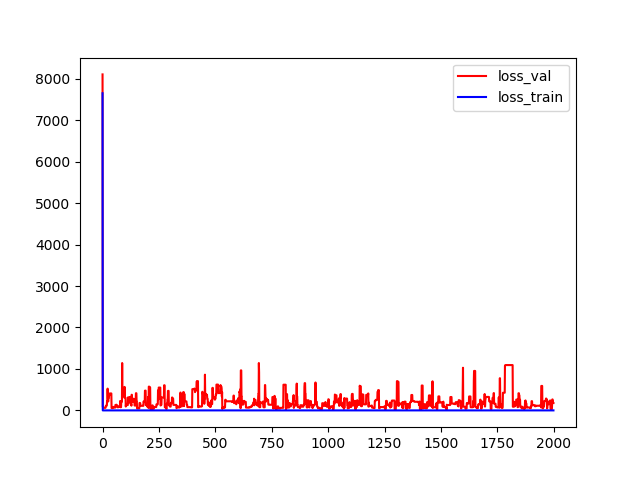
\includegraphics[width=2.5in]{loss2_aic.png}}
  \hspace{0in}
  \subfigure[loss for data 2(without the first 20\ points)]{
    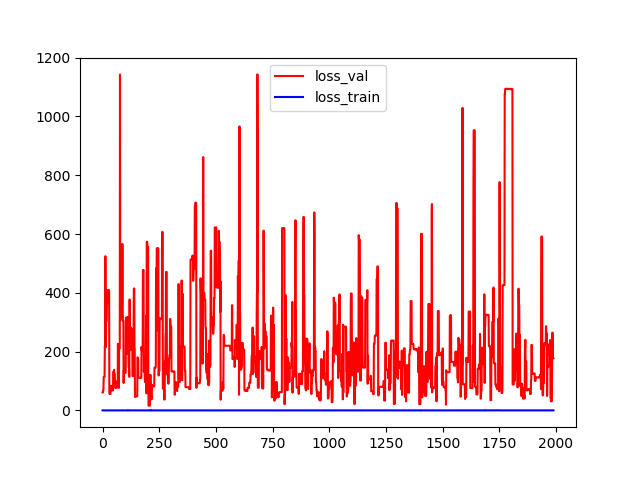
\includegraphics[width=2.5in]{newloss2_aic.png}}
  \caption{Loss Curve for RJMCMC-AIC method}
\end{figure}

对比loss曲线和数据表格,不难发现,使用AIC方法与使用RJMCMCSA方法得到的结果比较接近,其data1的训练结果和时间开销均要远好于data2的训练结果。不过对比AIC和SA方法的loss图象之后,我们可以清楚地看出本次实验中AIC的模型的稳定性要稍弱于使用SA算法取得的模型。

\subsubsection*{3. OLS}

OLS方法如IV.C所述,在本次实验中,分别在data1和data2的训练过程中取其截止条件中的$\rho$为$1e-4$和$5e-5$。

使用OLS方法在data1和data2两个数据集中分别进行训练,设置最大迭代次数为2000次。得到loss曲线如Figure 7中所示。将OLS方法分别在两个数据集上的时间开销及训练结果整理成Table 4,其中loss为最终模型在全部996个样本上的均方误差。

\begin{figure}[H]
  \centering
  \subfigure[loss for data 1]{
    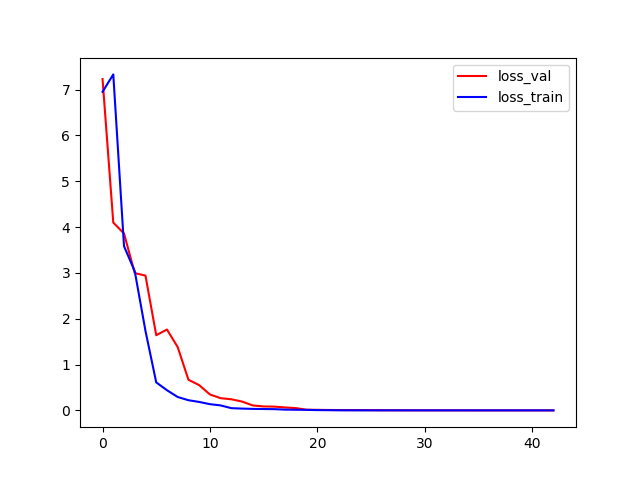
\includegraphics[width=2.5in]{loss1_ols.png}}
  \hspace{0in}
  \subfigure[loss for data 2]{
    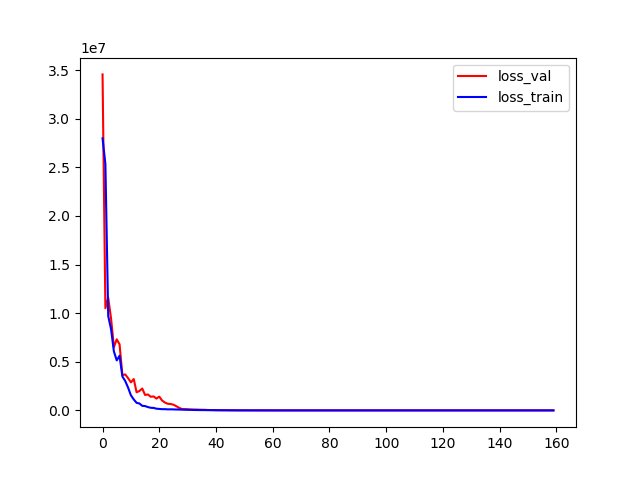
\includegraphics[width=2.5in]{loss2_ols.png}}
  \caption{Loss Curve for OLS method}
\end{figure}

从loss曲线中可以看出,OLS方法的稳定性较好,loss下降之后几乎没有太大的波动。且其训练所需时间要远小于使用RJMCMC方法的训练时间。

\subsubsection*{4. Discussion}

将3种方法在data1和data2数据集上的训练结果分别整理成Table 5和Table 6,从表中数据可以看出,在data1数据集上三种方法最终都能取得比较好的结果,而在data2数据集上三种方法则产生了较大的差异。

\begin{itemize}

\item OLS方法的收敛速度最快,在训练集和验证集上的loss比较接近,没有出现明显的过拟合情况,不过最后在全体样本上的测试结果不如SA和AIC与RJMCMC结合的方法。

\item 使用RJMCMC方法最后能取得一个优于OLS方法的模型,但容易出现比较明显的过拟合情况。训练集和验证集上的结果差异较大。在尝试了几次之后发现并不能将过拟合的情况消除。

\item 当数据模型比较复杂时,RJMCMC方法的稳定性不如OLS方法

\end{itemize}

\section*{\centering VI. Conclusion}

本文从原理和实际测试结果出发,详细分析了RJMCMC+SA\/AIC, OLS等几种重要的模型选择方法,从而对RBF网络模型自动选择技术给出了综合性地说明。几种方法各有利弊,在不同的应用场景中使用不同的选择方法可以取得更好的效果。

\section*{\centering Acknowledgement}

在这次的课程设计中,张静阳、全雨晗、李一卓等几位同学与我进行了多次深入的讨论,这让我对相关知识有了更细致的了解,在遇到不解的问题时他们也给予我许多参考意见。感谢他们的无私帮助。

当然也要感谢欧智坚老师以及两位助教的辛苦付出,这次作业有一定难度,不过在完成之后也能让我们有比较大的收获,感谢您们的悉心教导。

\renewcommand{\refname}{\hfil References}
\bibliographystyle{unsrt}
\bibliography{mybibtex}

\end{document}
